\documentclass[11pt,letterpaper]{article}

\usepackage{booktabs}
\usepackage{caption}
\usepackage{subcaption}
\usepackage{setspace}
\usepackage{hyperref}
\usepackage{multirow}
\usepackage{minted}
\usepackage{lineno}
% \linenumbers
\usepackage{pslatex}
\usepackage{apacite}
\usepackage{amsmath}
\usepackage{graphicx}
\usepackage[margin=1.0in]{geometry}

% \doublespace

\newcommand{\sigc}{\ensuremath{\sigma_c}}

\title{Effects of extremism and cultural environment on cultural polarization}

\author{Matthew A.~Turner}

\begin{document}

\maketitle

\abstract{An agent-based model is developed based on the opinion formation model of
\citeA{Flache2011}. The main innovation to the model of Flache and Macy is the addition of a
term representing the cultural influence on agents' opinions. Over 2,000 experiments
were performed. Experiments varied the strength of cultural influence as well
as limited how extreme agents initial opinions could be. Phase transitions emerged
that showed in some situations, culture has no effect on the final polarization
state of the system. Other phase transitions revealed that at a critical strength,
culture could induce polarization in a system with small-magnitude initial
opinions. This has practical applications for examining publically-available 
social data and guiding behavioral studies in the future. The work presented here
also suggests further
computational and analytic studies of the mechanisms of opinion formation and
the emergence of polarization in organizations and societies.

\vspace{0.25in}

Model, experiment, and visualization code can be accessed on GitHub:
\url{https://github.com/mtpain/polarization}
}

\section{Introduction}
\label{sec:Introduction}

Polarization of opinion in organizations is a fundamental feature of 
human society. While some difference in opinion is necessary, excessive polarization
can make organizations freeze. Opinion formation is a complex process, and
largely predetermined or unconscious. We are born in to communities that have
pre-existing opinions we often can't help but adopt ourselves. There are 
cultural forces constantly affecting our opinions, either consciously or
unconsciously. Of course, the opinions of members of our social networks 
influence our opinions as well.

A number of societal issues give rise to strong, differing opinions among a
population. Support for war, amenability to immigration, belief in climate change,
and support for political violence are some of the most pressing issues that 
threaten the peace and livelihoods of the people of the world. While the opinions
of those in our social networks have an impact on how we think about such issues,
the issues themselves arose from outside our social networks; these are features
of the world that demand our attention. Similarly, our reasoning about whether
or not we should go to war with another country, or any of the other issues
just mentioned, is largely affected by the pronouncement of politicians, 
media coverage, spin, and opinion, and events like terrorist attacks \cite{Martin2016}. 
\citeA{Kalmoe2014} showed that support for violent means for attaining political
ends increased among aggressive people when they were exposed to mildly violent
metaphors. Kalmoe also showed that the least aggressive among us lose faith in
the political system when exposed to the same metaphorical violence.
In the case of whether or not to ``believe in'' anthropogenic climate change, 
extreme weather events like superstorm Sandy can change people's minds \cite{Rudman2013}.

The purpose of the agent-based model presented here is to examine the relationship
between the evolution of polarization in a population as a function of 
influences from each agent's social network,
extremity of a population's initial opinions, and cultural effects outside of 
an agent's social network. Building on the model of cultural polarization of
\citeA{Flache2011}, I added an explicit term for cultural effects whose strength
of influence is varied. I also limited the extremity of opinion any given agent
can start with, so that the population's initial polarization is also limited.
The main result of \citeA{Flache2011} was that when populations are allowed to
have opinions of negative valence, taking values between -1 and 1, that polarization 
does indeed emerge. Polarization is maximized in a population when there are two
groups of agents of equal size, with every agent in each group sharing the
same opinions, and with each group's collective opinion being maximally opposed to 
the other group's. The degree of influence between agents is represented by a
weight which may be negative, or repulsive, 
which causes two agents' opinions to move further apart. Opinions become 
entrenched through the micro-level assumptions of the model.

Flache and Macy paid scant attention to the dynamics of polarization, possibly
because in that model the dynamics are not too interesting between different
configurations they considered. By varying the two parameters I introduce,
maximum initial opinion magnitude and the magnitude of cultural effects, rich
dynamics emerge. Extreme initial opinions lead to frozen polarization measures
that cultural effects cannot move. For more modest initial opinions, cultural
effects have no effect up to a point, but eventually drive the system to 
a highly polarized final state. In the intermediate strength of cultural 
effects, the final polarization of the system is uncertain. When the system does
attain some nonzero polarization, it is not to a fully polarized state, but
only partially polarized. I demonstrate that the structure of the phase 
transition along the strength of cultural effects is more or less the same
up to a certain extremity of initial opinion. This structure is destroyed once
initial opinions become too extreme. 

By examining the details of these transitions in final state of polarization,
we can gain insight into the dynamics of polarization in populations. This
opens the door to modeling real systems where initial extremism and cultural
effects can be quantified. In the long run, this could guide management and
communication strategies that leads to optimal levels of polarization in 
organizations of all sizes and forms.

\section{Methods}
\label{sec:Methods}

\subsection{Model}
\label{sub:Model}

This model extends the cultural polarization model introduced by 
\citeA{Flache2011}. In this model, agents are nodes of a graph with weighted
edges connecting neighbors. Each agent, indexed by $i$, has a set of $K$ opinions 
that change over time, $s_{i,t} = \left\{ s_{ik,t} | k = 1, \ldots, K\right\}$.
Edge weights are updated at each iteration. The weight
at time $t+1$ between agents $i$ and $j$ are given by 

\begin{equation}
  w_{ij,t+1} = 1 - \frac{1}{K} \sum_{k=1}^K \left| s_{jk,t} - s_{ik,t} \right|
\end{equation}

\noindent
If agents $i$ and $j$ have exactly the same $K$ opinions, $w_{ij} = 1$. 

Opinions are updated through a weighted difference of their opinions. 
First an unscaled difference is calculated for each agent's opinions at a given time

\begin{equation}
  \Delta s_{ik,t} = \frac{1}{2 |\mathrm{n}_t(i)|} 
    \sum_{j \in \mathrm{n}_t(i)} w_{ij,t} \left(s_{jk,t} - s_{ik,t}\right) + \epsilon(\sigc)
\end{equation}

\noindent 
where $\epsilon(\sigc) \sim \mathcal{N}(0, \sigc)$. One innovation on the
model of \citeA{Flache2011} is this noise term. In the experiments,
$\sigc$ will be varied to represent random effects due to the cultural environment
and an agent's random variation of opinions.
$\mathrm{n}_t(i)$ is the number of neighbors of agent $i$ at time $t$.
This difference is scaled to be less the closer $|s_{ik,t}|$ is to 1. At $t+1$
each opinion is updated,

\begin{equation}
  s_{ik,t+1} = \begin{cases}
                  s_{ik,t} + \Delta s_{ik,t}\left(1 - s_{ik,t}\right) 
                      \quad \mathrm{if}~ s_{ik,t} > 0 \\
                  s_{ik,t} + \Delta s_{ik,t}\left(1 + s_{ik,t}\right)
                      \quad \mathrm{if}~ s_{ik,t} \leq 0.
  \end{cases}
\end{equation}

\noindent
Note that as $s_{ik,t} \rightarrow \pm 1$, opinions will be increasingly 
entrenched. This is a major mechanism for the emergence of polarization in the
population. 

Polarization is defined to be the scaled variance of differences between all
agents in the population. 

\begin{equation}
  P_t = \frac{1}{N(N-1)} \sum_{i=1}^{N} \sum_{j>i}^{N} \left(d_{ij,t} - \bar{d_t}\right)^2.
\end{equation}

$d_{ij,t} = \frac{1}{K} \sum_{k=1}^K \left|s_{jk,t} - s_{ik,t}\right|$ is the
average opinion difference across $K$ opinion dimensions. The average of $d_{ij,t}$
across all pairs $i,j$ is $\bar{d_t} = \frac{1}{N(N-1)} \sum_{i=1}^{N} \sum_{j>i}^{N} d_{ij,t}$.


\subsection{Experimental Setup}
\label{sub:Experimental-Setup}

Using this framework, I performed an experiment to test the influence of the
initial magnitude of any opinion, plus the influence of the magnitude of 
random cultural influences, represented by the standard deviation $\sigc$.
Initial magnitude of opinion just means limiting the absolute value of any 
opinion. Representing the maximum initial magnitude of opinions by $S$, 
the initial conditions could be written $|s_{ik,t=0}| \leq S$. An illustration
of the effect of the maximum initial opinion magnitude, $S$, is shown in
Figure \ref{fig:initial-opinion-example}. By 
analyzing many combinations of the parameters, $(S, \sigc)$, we can 
identify phase shifts in the polarization measure of the system. From this, we
can infer what level of initial magnitude of opinion and magnitude of cultural
influence lead to either polarized or unpolarized systems. Note that all 
experiments in \citeA{Flache2011} had $S = 1$ and $\sigc = 0$.
For every pair of $(S, \sigc)$, the model evolved over 1000 iterations.
Ten trials were run for each parameter pair. 

\begin{figure}
  \centering
  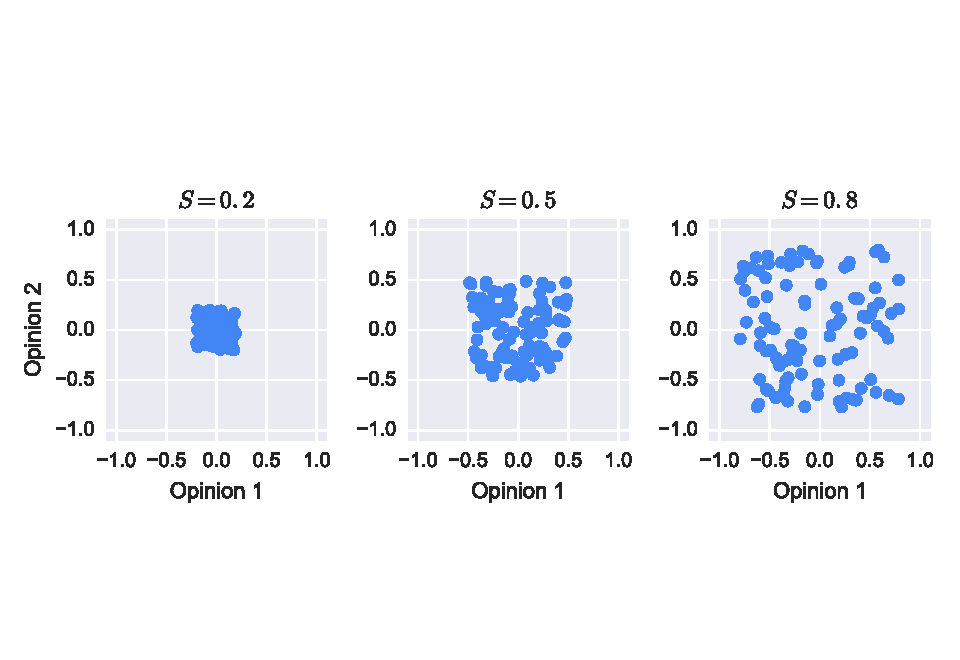
\includegraphics[width=0.8\textwidth]{figures/initial-opinion-example.pdf}
  \caption{The maximum initial opinion magnitude, $S$, limits the magnitude of
  an opinion in any of the $K$ opinion dimensions. Shown here is the initial
  distribution of agent opinion vectors for our experiments where $K=2$. $S$
  limits each dimension to a square of width $2S$ centered on the origin.}
  \label{fig:initial-opinion-example}
\end{figure}

\section{Results}
\label{sec:Results}

Now we will journey into the dynamics of polarization revealed by the experiments.
The first stop on this journey is the global phase diagram, shown in Figure
\ref{fig:phase-diagram}. Here we can see some clear regions where the system
consistently converges to either a totally unpolarized or polarized state.
Where the initial extremism, $S$, is less than 0.75 and the 
cultural effects magnitude, $\sigc$, is less than 0.06, the system
reliably converges to an unpolarized state, or $P=0$. The system converges to
a highly polarized state, $P > .8$, for $S < 0.75$ and $\sigc > .14$. 

\begin{figure}
  \centering
  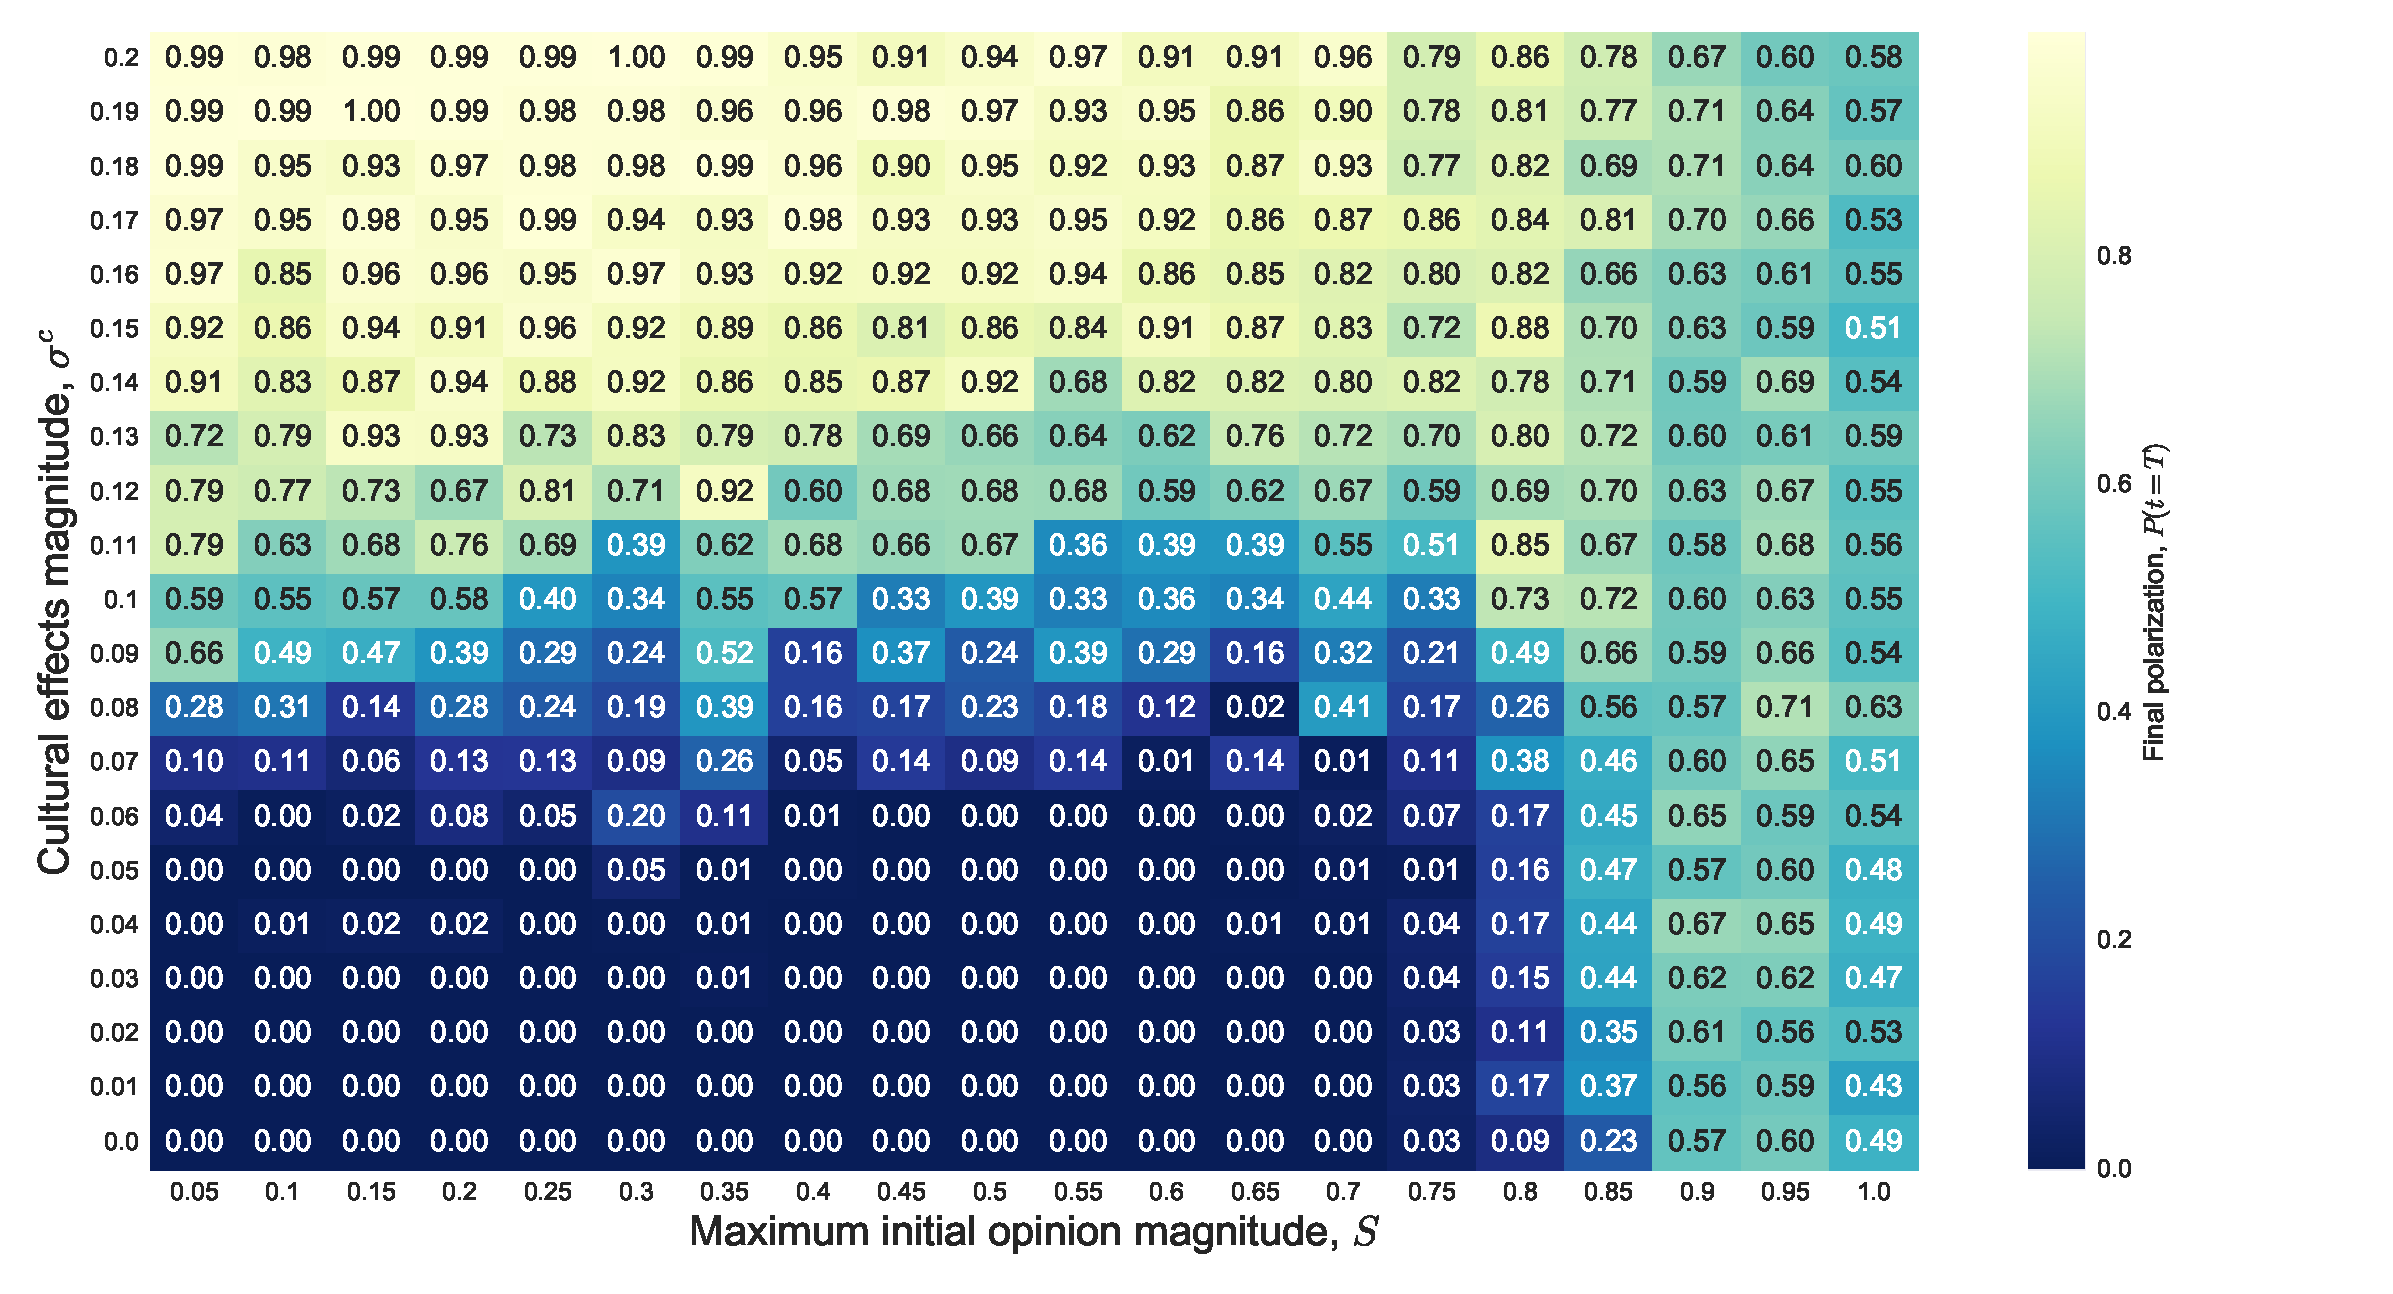
\includegraphics[width=\textwidth]{figures/phase-diagram.pdf}
\caption{The final polarization of the population changes as a function of
  the maximum initial opinion magnitude, $S$, and the strength of cultural
  effects, $\sigma_c$. Before $S\approx0.85$, small intial differences of
  opinion are radicalized with increasing cultural effects. 
  After $S\approx0.85$, cultural effects have little impact on the final 
  value of polarization.}
\label{fig:phase-diagram}
\end{figure}

This phase diagram deserves more investigation. First, we should look into
the dynamics of polarization for some $(S, \sigc)$ pairs. Consider the 
column of the phase diagram in Figure \ref{fig:phase-diagram} with 
$S=0.55$. Between $\sigma_c=0.11$ and $\sigma_c=0.12$, the average polarization
goes from .36 to .68. To get an understanding for these average values, 
see Figure \ref{fig:series}, which shows the evolution of the system over 
1,000 iterations for ten trials. Each trial is shown in a different color.
At $\sigc=0.08$, all but three trials converge to $P=0$. Two trials converge to
$0 < P < 0.5$, and one trial converges to a large polarization, $P\approx0.85$.
Compared to the other values of $\sigc$, when the system does evolve to a
non-zero polarization it takes significantly longer to reach that non-zero
polarization. When $\sigc=0.10$, more simulations result in $P>0.5$, but still
the rise to equilibrium polarization takes longer than those simulations in
the final plot, Figure \ref{fig:series}c, with $\sigc=0.16$. This final plot
shows that all iterations converge to a large polarization with equilibrium
reached in about 200 iterations, compared with 600-1000 iterations for the
other two values of $\sigc$.

\begin{figure}
  \centering
  \begin{subfigure}[b]{\textwidth}
    \centering
    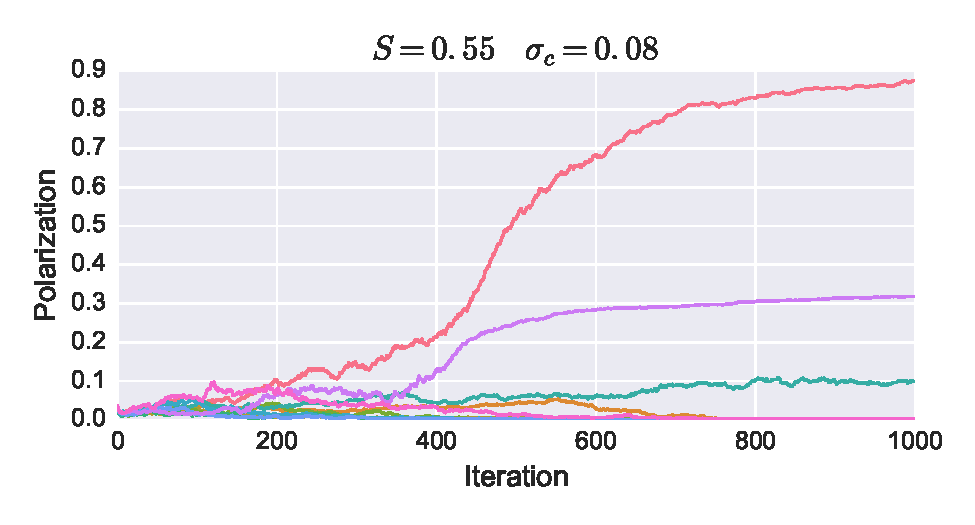
\includegraphics[width=.7\textwidth]{figures/s-0d55_sc-0d08_series.pdf}
    \caption{Only one trial reaches high polarization}
  \end{subfigure}

  \begin{subfigure}[b]{\textwidth}
    \centering
    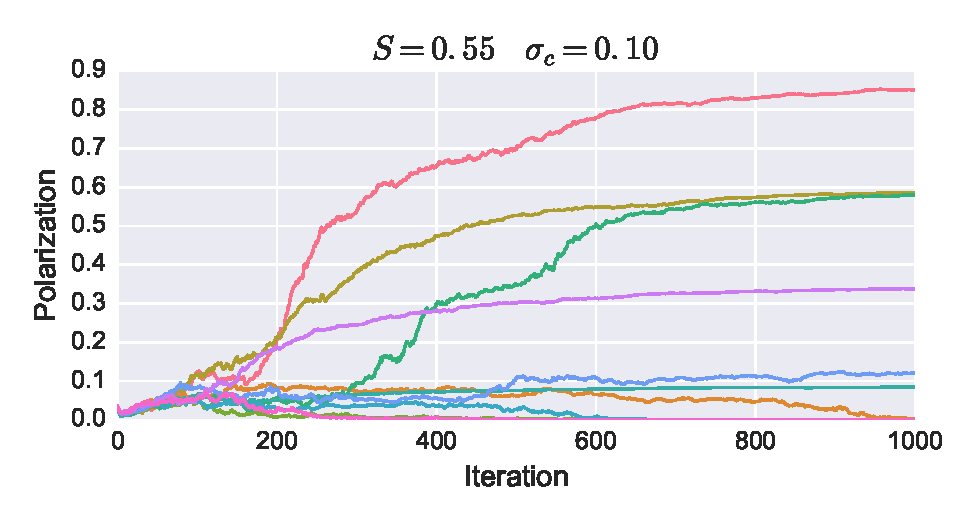
\includegraphics[width=.7\textwidth]{figures/s-0d55_sc-0d10_series.pdf}
    \caption{Three of the trials result in polarization greater than .5}
  \end{subfigure}

  \begin{subfigure}[b]{\textwidth}
    \centering
    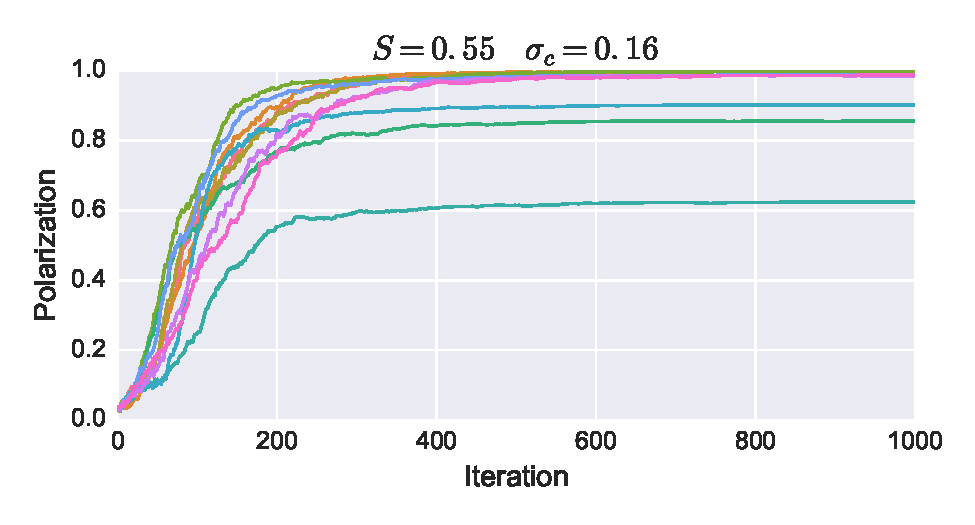
\includegraphics[width=.7\textwidth]{figures/s-0d55_sc-0d16_series.pdf}
    \caption{All trials achieve polarizations above .5}
  \end{subfigure}
  \caption{The probability of full polarization increases with the strength of
    cultural effects. Each line color represents one of the ten trials. For
    the two smaller values of $\sigc$, when the trials do reach a polarization
    greater than .5 they arrive slower than $\sigc=1.6$.}
    \label{fig:series}
\end{figure}

With a better understanding of the time-evolution of these systems across trials,
we can move on to investigate the average polarization over trials for
various values of $\sigc$. As suggested by Figure \ref{fig:phase-diagram}, 
the rise from unpolarized final states to polarized final states over $\sigc$
is similarly structured, sigmoidal, when $S < .8$. This structure decays
when $S \geq .8$. This behavior is shown in Figure \ref{fig:phase-transitions-by-culture}.
Along with the average polarization over trials, the variance is represented
by error bars in each of the two plots in Figure \ref{fig:phase-transition-by-culture}.
What the plot in the global phase diagram of Figure \ref{fig:phase-daigram}
could not show was the structure in the variance of polarization across $\sigc$.
This variance gives us another measure for further establishing the presence
of a phase transition. Instead of a phase transition in polarization, we 
see a phase transition to a lack of freedom for the system to evolve to either
an extreme polarized state, no matter what the value of $\sigc$. In other words,
we will see that extreme initial opinions lead to a situation where no amount
of cultural influence can alter the final state of polarization.

\begin{figure}
  \centering
  \begin{subfigure}[b]{\textwidth}
    \centering
    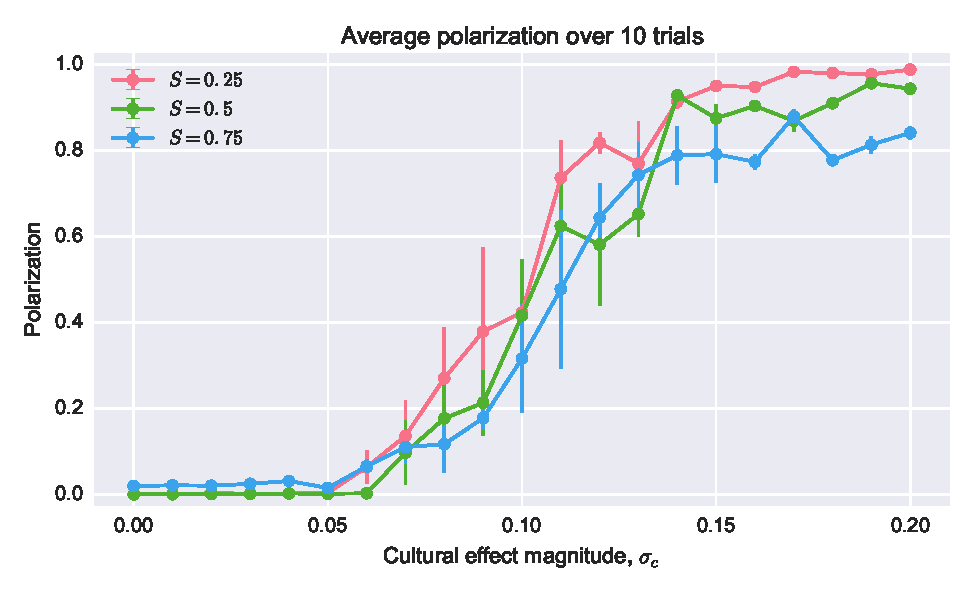
\includegraphics[width=.9\textwidth]{figures/pol-by-culture-25-5-75.pdf}
    \caption{When $S < .8$, polarization follows a sigmoid with increased
    variance for middle values of $\sigc$.}
  \end{subfigure}

  \begin{subfigure}[b]{\textwidth}
    \centering
    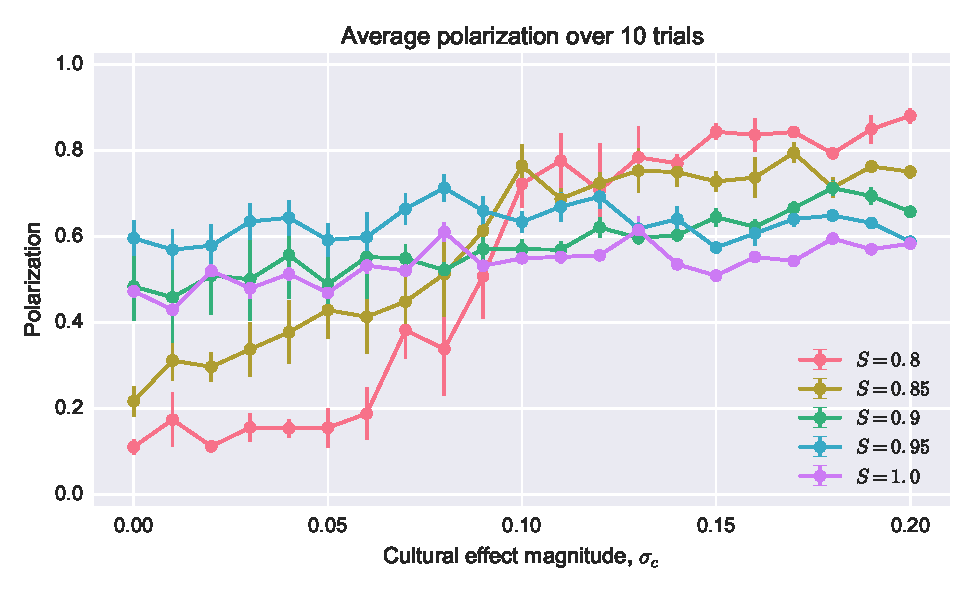
\includegraphics[width=.9\textwidth]{figures/pol-by-culture-8-85-9-95-100.pdf}
    \caption{When $S \geq .8$, the sigmoidal structure gives way to constant
    polarization across all cultural effect magnitudes, $\sigc$.}
  \end{subfigure}

  \caption{Phase transitions from unpolarized to polarized for a few values
    of maximum initial opinion magnitude, $S$. Phase transitions begin to 
    disappear when $S \geq .8$. When $S < .8$, polarization undergoes a 
    phase transition. There is increased variance over different trials 
    for intermediate polarization values, as illustrated in Figure \ref{fig:series}.
    }
  \label{fig:phase-transitions-by-culture}
\end{figure}

But how should we measure the structure of the variance? When the variance
of polarization over trials is plotted against $\sigc$, it appears to be
roughly quadratic once a critical $\sigc$ is reached. The strategy, then, is
to fit a quadratic polynomial to the variance, with one root being the last
$\sigc$ for which the variance is zero. The other root of the quadratic is
to be determined based on the fit. The measure we use for structure is the
difference between the two roots. An illustration of this method is shown in
Figure \ref{fig:quadfits}. For $S=0.25$, $S=0.5$, and $S=0.75$, it is possible
to fit a somewhat reasonable parabola to the variance. However, the structure
in the variance breaks down for $S=0.9$. 

\begin{figure}[h!]
  \centering
  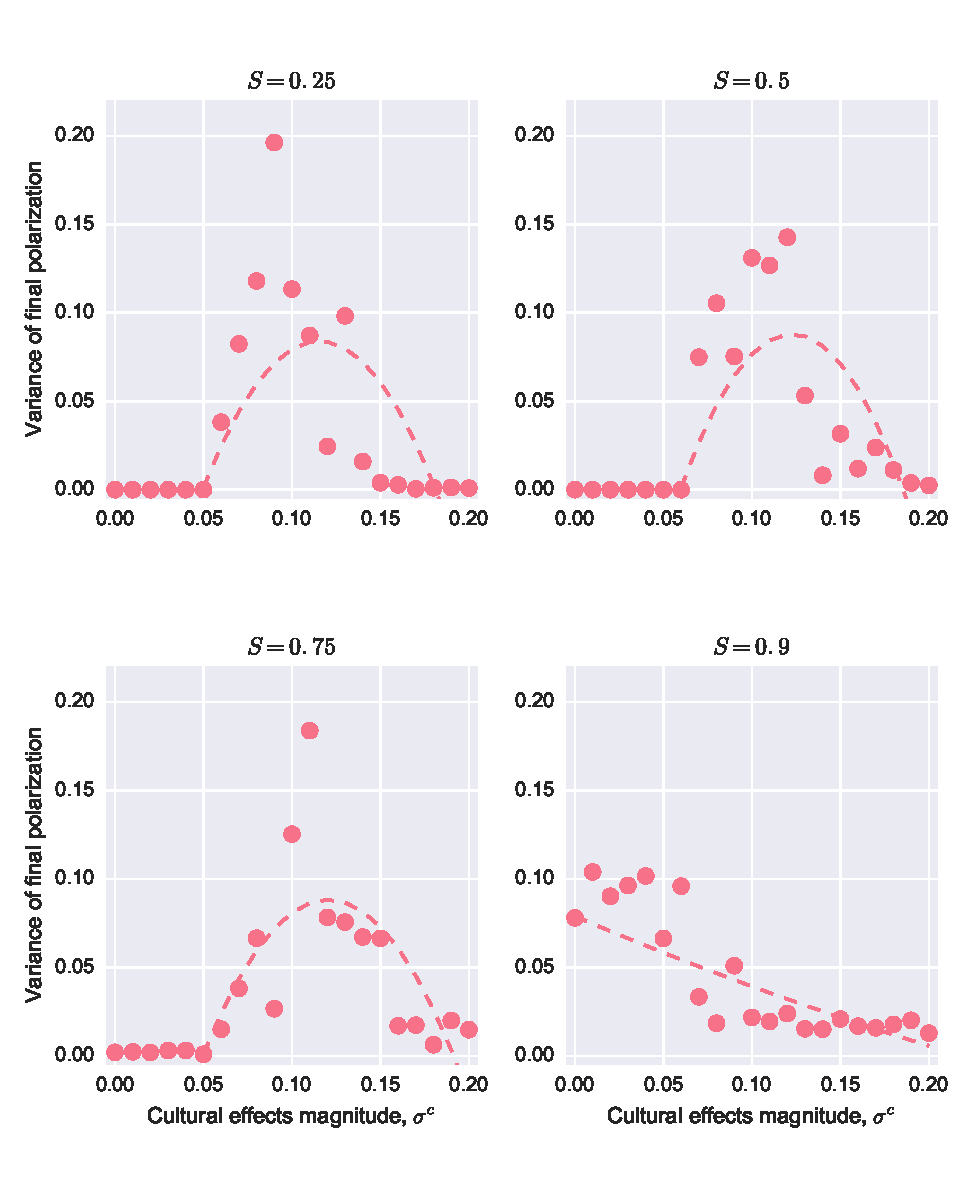
\includegraphics[width=\textwidth]{figures/quad-fits.pdf}
  \caption{Quadratic fits (dashed line) to the variance (dots) over all iterations for 
  various values of $S$. We can use the change in distance between roots of this
  quadratic fit as $S$ increases as a heuristic to observe phase transitions
  from sigmoidal structure in polarization over $\sigc$ to median polarization
  when $S > .8$.}
  \label{fig:quadfits}
\end{figure}

I call this distance between roots of the parabola the \textit{transition width},
as it is roughly the width of the transition in terms of $\sigc$ from 
a guaranteed unpolarized final state to guaranteed polarized final state. The
sudden jump of transition width as $S$ increases will indicate the phase 
transition from culture-dependent to culture-independent polarization. This
confirms what we already expected, that there is such a transition. But the
change in transition width is drastic, as shown in Figure \ref{fig:transition-widths}.
We see that the transition width holds almost constant until $S=.7$, when 
the width gradually increases until $S=0.85$. At $S=0.9$, the transition width
diverges, and varies greatly for $S \geq 0.9$.

\begin{figure}[h!]
  \centering
  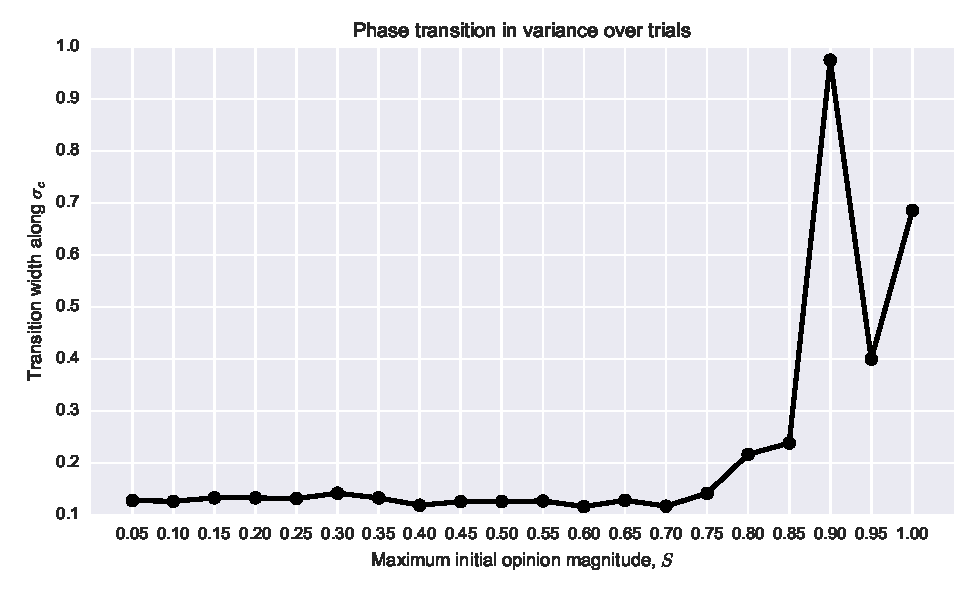
\includegraphics[width=\textwidth]{figures/transition-widths.pdf}
  \caption{Phase transition in the behavior of variance across trials. The
  profile of variance across $S$ is nearly constant until $S\approx0.8$. After
  this the structure of transition of the population from unpolarized to 
  polarized is destroyed by large initial opinions that do not change as the
  system evolves.}
  \label{fig:transition-widths}
\end{figure}


\section{Discussion}
\label{sec:Discussion}

By introducing a limit on the initial extremism of a population and the
extent to which culture influence opinion, we identified where cultures will
either homogenize or polarize. When the magnitude of the agents' initial 
opinions became too great, the final polarization was not independent of 
cultural influences. A region of uncertainty was also identified where
initial extremism and strength of cultural influence could not reliably predict
the final level of polarization. The presence of such a region indicated that
the system was sensitive to cultural influences. The absence of a region in
$(S, \sigc)$ space indicated the system was not sensitive to cultural 
influences: instead, agents initial opinions did not change much as the 
system evolved.

These results were obtained by simply restricting the magnitude of the 
agents' initial opinions and adding a gaussian noise term to the raw opinion update
equation from \citeA{Flache2011}. Taking the standard deviation of this noise
to represent the strength of influence of culture gave us a parameter to 
change. Although the modifications were simple, they provide a framework for
both behavioral experiments and a framework for analyzing real-world data.
One could imagine a behavioral experiment where participants were selected based
on their current opinions. Then participants could be grouped together to 
reflect various values of initial extremism, represented by $S$ in this study.
While the participants susceptibility to ``cultural effects'' might be difficult
to control for, it would be possible to give the participants evidence or 
arguments for or against a particular opinion on a set of issues. The evidence
or arguments could be made more or less forceful by pragmatic choices of 
language. The mix of forcefulness in communications could be manipulated to 
match various values of $\sigc$, the magnitude of cultural effect in this model.
Participants would be assigned neighbors to interact with according to the 
randomized caveman social network of this model.

As for analyzing real-world data available now, numerous studies have measured
polarization through natural language processing, publically-available 
demographic data, or a combination of the two. \citeA{Morales2015} proposed
a model of polarization, then applied it to measure political polarization 
in Venezuela after the passing of Venezuelan president Hugo Chávez. Using 
geotagged twitter data, the authors were able to partition geographic contours
of opinion in the captial, Caracas. \citeA{Gentzkow2015} studied polarization
in speeches in the United States congress from 1873 to 2009. They posit that
``innovation in political persuasion beginning with the \textit{Contract with
America}, possibly reinforced by changes in the media environment'' caused
the relatively recent increase in the degree of partisanship they observed. 
Perhaps the model presented in this paper could address the inverse problem of
finding a quantitative estimate of the strength of cultural influence given
the observed polarization. \citeA{Martin2016} study the effect of cable news
partisanship on voting behavior, finding that ``Fox News increases Republican
vote shares by 0.3 points among viewers induced into watching 2.5 additional
minutes per week.'' 

A major shortcoming of the model presented here is that there is only one 
species of agent. The study of political polarization in Venezuela, \citeA{Morales2015},
considered two species of agent: ``elites'' and ``listeners''. Such a system
should be explored in the model developed here. Elites would represent 
politians, political organizations, and media outlets. The opinions of these
elites would not change, only influence others' opinions. These elites might also
have more neighbors than listener agents to better represent the real-world
situation. We could also more explicitly encode biased processing of information
by making the cultural impact term $\epsilon \sim \mathcal{N}(\mu_c, \sigma_c)$,
where $\mu_c \in [-1, 1]$ would be different for each agent and represent that agents
bias towards one valence or another on a certain opinion. 

We have only considered $K=2$-dimensional opinion vectors for agents. Other values of
$K$ should be tested to see if the same phase transitions are observed. Another
scaling issue is the number of agents. This work has only studied $N=100$. Are
similar phase transitions observed for other values of $N$? If not, what effect
does population size have on the system dynamics.

We are also lacking any sort of analytical results that could help us more 
deeply understand the reason for the observed phase transitions. One reason
analytical methods are difficult is that opinion updates are done asynchronously,
with each agent updating its opinion in a random order at every timestep. 
So the same initial conditions for a simulation will not, in general, converge
to identical final polarization states. \citeA{Dandekar2013} shows that the
DeGroot model of opinion formation can never be polarizing. They advise 
``polarization is not a property of a state of society; instead it is a 
property of the dynamics through which individuals form opinions.'' In this model,
a sufficiently simple yet representative process should be identified. Then,
following their lead, we can calculate whether or not the opinion process
here is polarizing or not. The results presented in this current work suggest
that polarization will have to be graded. That is, I have showed that polarization
often converges to a value between 0 and 1, not totally polarized or unpolarized.

In all, these challenges represent varied and hopefully fruitful avenues for
future work. Simple rules give rise to rich structure. Such structure gives us
footholds for quantification of behavior and communication. As we understand 
more about the conditions that give rise to harmful polarization, we can identify
steps to move towards healthier levels of polarization. Such study is also 
fundamentally interesting, as the emergence of extreme opinions is a central
feature of human society.

\newpage

\bibliographystyle{apacite}

\setlength{\bibleftmargin}{.125in}
\setlength{\bibindent}{-\bibleftmargin}

\bibliography{/Users/mt/workspace/papers/library.bib}


\end{document}
